\documentclass[11pt,a4paper]{article}
\usepackage[ngerman]{babel}							% enables Hyphenation for german
% \usepackage[babel, german=quotes]{csquotes}
\usepackage{subfigure}								% enables subfigures
\usepackage{amsmath}								% enhances math output
\usepackage{amsfonts}								% additional math fonts
\usepackage{graphicx}								% alternativ graphic interface
\usepackage{color,listings}	 						% codesequences 
\usepackage{import}
\usepackage{cite}
\usepackage{enumitem}
%löst Probleme mit ä,ö,ü
\usepackage[utf8]{inputenc}
%\usepackage[T1]{fontenc}
%Deutsche Silbentrennung
\usepackage[ngerman]{babel}
% \usepackage{biblatex}
\usepackage{fancyhdr}			%% fuer Pagestyle fancyhdr mit eigenen Kopf und Fusszeilen


\author{Heinz Hofmann und Jonas Schmid}

%% Pagestyle mit eigenen Kopf und Fusszeilen
\pagestyle{fancy}
\fancyhf{}								%% leerraeumen
% \fancyhead[L]{\includegraphics[height = 20pt]{logo.png}}
% \fancyhead[R]{Simulationstools}
\renewcommand{\headrulewidth}{0.0pt}	%% obere Trennlinie
% \fancyfoot[C]{\thepage}					%% Seitennummer
\fancyfoot[L]{Heinz Hofmann und Jonas Schmid}	
\fancyfoot[R]{20. Dezember 2017}		
\renewcommand{\footrulewidth}{0.4pt}	%% untere Trennlinie


\begin{document}

\section*{ \center \textbf{\LARGE Algorand: Eine vielversprechende Blockchain basierte Kryptow\"ahrungen}}
% \center \textbf{\LARGE Algorand: Eine vielversprechende Blockchain basierte Kryptow\"ahrungen} \\

Die populärsten Blockchain basierten Kryptow\"ahrungen wie Bitcoin und Ethereum haben noch einige technische M\"angel.
Insbesodere der Energieverschwenderischen Proof-of-Work kann auch wegen den grossen 
und damit m\"achtigen Mining Pools zum Problem werden.
Zudem stossen Bitcoin und in absehbarer Zeit auch Ethereum an ihre Kapazit\"atsgrenzen (Transaktionen pro Zeit).
Einige Leute um den MIT Professor und Turing Award Winner Silvio Micali haben die alternative Cryptow\"ahrung Algorand entwickelt.
Diese soll eine deutlich gr\"ossere Kapazit\"at bereitstellen als bisherige Blockchain basierte L\"osungen und anstelle von Proof-of-Work wird ein Proof-of-Stake Verfahren angewandt.
Algorand befindet sich noch im Entwicklungsstadium und wird deshalb noch nicht in der Praxis eingesetzt.
Es wurde jedoch erfolgreich ein Prototyp mit einigen hunderttausend Nodes simuliert\cite[Kapitel Implementation \& Evaluation]{Gilad:2017:ASB:3132747.3132757}.
Dabei wird eine "Transaction Confirmation Time" von rund einer Minute erreicht und es k\"onnen rund 125 mal mehr Transaktionen get\"atigt werden als bei Bitcoin \cite[Introduction]{Gilad:2017:ASB:3132747.3132757}.
Die zur Verf\"ugung stehenden Quellen sind gr\"ossten Teils auf ein Team im CSAIL am MIT zur\"uckzuf\"uhren. % Computer Science and Artificial Inteligence Laboratory
Nachfolgend beziehen wir uns deshalb mehrheitlich auf das Paper \cite{Gilad:2017:ASB:3132747.3132757}, 
welches Algorand resp. den Algorithmus detailiert unserer Meinung nach sehr gut beschreibt,
ein grober \"Uberblick wird im Abschnitt Overview oder im Betrag \cite{ScalingConsensus} gegeben.
Die Offenen Punkte und Probleme werden im Paper auch gut beschrieben.

\section*{\"Ubersicht}
Algorand basiert auf einer Blockchain sehr \"ahnlich wie Bitcoin.
Um Konsens bez\"uglich des jeweilig n\"achsten Blockes zu erreichen,
wird der n\"achste Block resp. der jeweilge Erzeuger mittels Byzantine Agreement ermittelt.
Ein komplettes Byzantine Agreement mit allen Nodes ist jedoch wegen des viel zu hohen Kommunikationsaufwandes nicht durchf\"uhrbar.
Desshalb aggiert bez\"uglich Byzantine Agreement immer nur ein Subset von Nodes\footnote{Beim Algorand Prototypen wurden 26 Nodes angestrebt.}.
F\"ur jede Kommunikationsrunde werden die Rollen mittels Cryptographic Sortition verteilt.


\newpage
% \chapter{\textbf{\Large Block zur Blockchain hinzuf\"ugen }}\\
\section*{N\"achsten Block ermitteln}
Das Hinzuf\"ugen eines Blocks zur Blockchain vollzieht sich in drei Steps.
\begin{enumerate}[label=\arabic*)]
	\item \textbf{Block erzeugen und broadcasten}\\
	\textbf{Jeder} Node f\"uhrt bei sich die Sortition durch, um herauszufinden, ob er einen Block broadcasten darf. 
Falls ja f\"ugt er alle Transaktionen, die er m\"ochte dem Block hinzu und "broadcasted" diesen dem Netzwerk. 
Er wird einer von ca. 26 Nodes sein, der einen Block broadcasten darf. 
Jeder dieser ca.26 gebroadcasteten Bl\"ocke hat aber eine gewisse Priorit\"at, welche ebenfalls durch die Sortition erzeugt wurde.
	 
	\item \textbf{Byzantine Agreement}\\
	Nun wird in zwei Substeps das Problem \grqq{}einen aus vielen Bl\"ocken ausw\"ahlen\grqq{} auf das bin\"are Problem \grqq{}entweder den proposten Block oder einen leeren Block auszuw\"ahlen\grqq{} reduziert.
	\begin{enumerate}[label=\Roman*)]
		\item Nach einer bestimmten Wartezeit(zur Synchronisation) gibt ein \textit{Gremium} von zuf\"allig durch Sortition ausgew\"ahlten Nodes eine Stimme f\"ur je einen Block ab. Sie w\"ahlen jeweils von den f\"ur sie sichtbaren Blocks denjenigen mit der h\"ochsten Priorit\"at. Diese Stimme broadcasten Sie wieder durch das Netzwerk.
		
		\item Ein erneut durch Sortition zuf\"allig gew\"ahltes Gremium wartet bis entweder gen\"ugend Votes f\"ur einen Block zusammenkamen, oder bis eine bestimmte Zeit abgelaufen ist. 
		Sind gen\"ugend Votes zusammengekommen, wird der entsprechend gew\"ahlte Block promotet.
		Ist die Zeit abgelaufen, wird ein leerer Block promoted. 
		Alle gutartigen Nodes werden hier entweder denselben vollen Block oder einen leeren Block promoten. 
	\end{enumerate}
	\item \textbf{Binary Byzantine Agreement}\\
	Ab hier wird in einem Bin\"aren Byzantinischen Verfahren entweder der eine "volle" Block oder der leere Block gew\"ahlt. 
	Falls es keine fehlbaren Nodes gibt ist dieser Prozess in wieder zwei Substeps beendet.
	Wird der Prozess aber von Fehlbaren Nodes gezielt mit z.B. Broadcasts von falschen Bl\"ocken gest\"ort(Was sehr schwierig ist, weil diese Nodes ins Gremium h\"atten gew\"ahlt werden m\"ussen) kann dieser Vorgang bis zu 9 Substeps andauern.
	In jedem Substep wird jeweils ein neues Gremium gew\"ahlt, welches aufgrund der Vergangenheit Votes f\"ur den einen vollen oder einen leeren Block abgeben. 
	Jeder Dritte dieser Substeps wird ausserdem eine "gemeinsame" M\"unze geworfen, welche hilft Fortschritt zu garantieren. 
\end{enumerate}
Dieser ganze Prozess dauert ca. 20 Sekunden. Konservativerweise wurden die Wartezeiten der Nodes, bis sie voten so gew\"ahlt, dass dieser ganze Prozess rund eine Minute dauert.

\begin{figure}
	\centering
	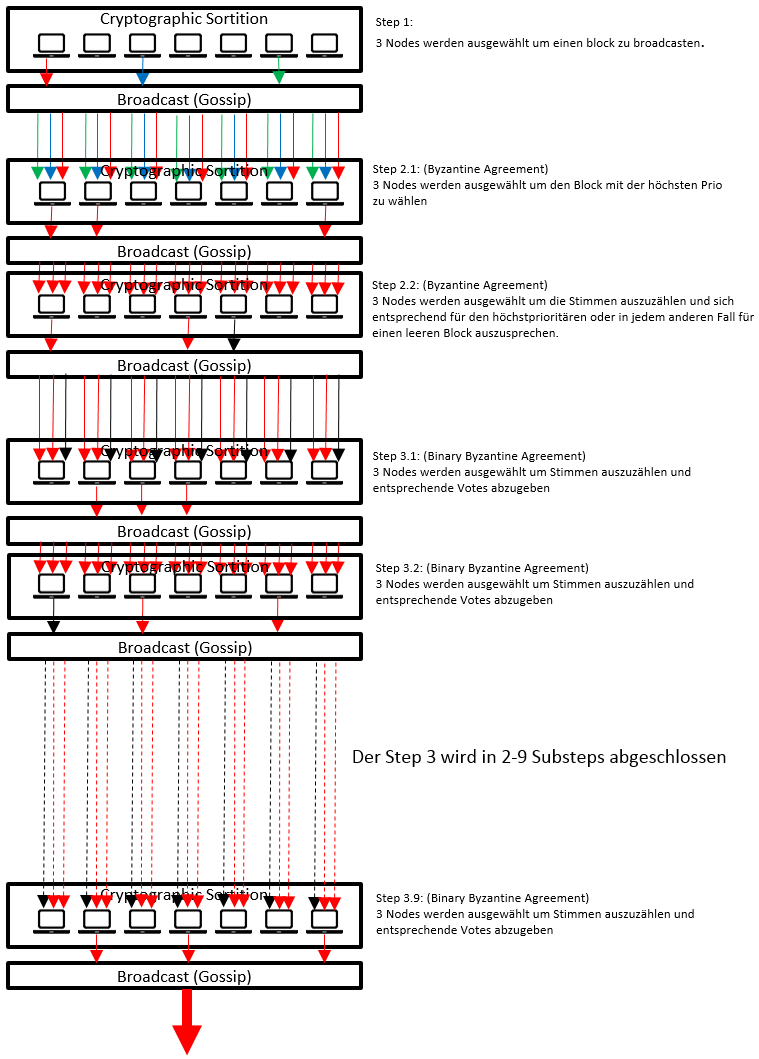
\includegraphics[scale=0.65]{Algorand.png}
	\caption{Dies ist eine Grafik als pdf}
	\label{img:grafik-dummy2}
\end{figure}



\section*{Cryptographic Sortition}
% \chapter{\textbf{\Large Cryptographic Sortition}}\\
F\"ur jede Kommunikationsrunde berechnet jeder Node f\"ur sich ob er f\"ur ein oder mehrere Mandate (Block broadcasten oder Gremium) gew\"ahlt ist.
Dazu wird mittels \textit{verifiable random function}, kurz VRF, aus dem \textit{private key} und einem bekannten \textit{seed} ein \textit{hash} und ein Beweis $\pi$ berechnet.
Die Mandate werden abh\"angig vom jeweiligen Balance und berechnetem Hash der Nodes verteilt.
Das heisst ein Node welcher viel Geld im System hat, bekommt \"ofter ein Mandat zugeteilt, als ein Node welcher wenig Geld im System hat.
Somit ist das Auswahlverfahren vom Typ Proof-of-Stake und sch\"tzt Algorand vor \textit{Sybill attacks}.
Der \textit{seed} ist jeweils abh\"angig von der vorangehenden Kommunikationsrunde.
Weiter wird mit dem Hash jedem Node eine Priorit\"at zugeteilt, welche f\"ur das Byzantine Agreement verwendet wird.
Die VRF ist so konzipiert, dass der Hash nur mittels Private Key berechnet werden kann.
Somit kennt keiner die ausgew\"ahlten Nodes, bevor diese eine Mitteilung ins Netztwerk versendet und
damit ihr Mandat ausgef\"uhrt haben.
Damit ist ein Agriff auf nur diese wenigen Nodes nicht m\"oglich.
Mit dem Beweis aus der VRF und dem jeweiligen Public Key kann jeder Node jeden Hash und damit die Rollenzuteilung jedes Nodes \"uberpr\"ufen.

% \bibliographystyle{plain}
\bibliographystyle{apalike} % makes reference labels like [Redmond et al., 2016]
\bibliography{algorand}{}



\newpage

\chapter{\textbf{\Large Trash}}\\

\paragraph*{Empfehlung f\"ur eine Vorlesung oder Seminar}
Das Paper \cite{Gilad:2017:ASB:3132747.3132757} w\"urde sich gut eignen f\"ur eine weitere "Buchdiskussion".
Es werden einige Aspekte bez\"uglich Distributed Systems/Ledger aufgegriffen welche
im Buch "Distributed Ledger Systems" von Roger Wattenhofer tematisiert wurden, z.B. Byzantine Agreement.

Falls nun ein b\"osartiger Node in dieser Position verschiedene Bl\"ocke oder einen fehlerhaften Block
verteilt, kann sich das \textit{commitee} nicht einigen und erweitert die Blockchain um einen leeren Block ohne Transaktionen.

Dabei wird jeder neue Block durch ein Committee bestehend aus weniger als 100 Nodes mittels Byzantine Agreement zusammengestellt resp. ausgew\"ahlt.
Das Committee wird zuf\"allig aber gewichtet mit den jeweiligen Balances der Nodes f\"ur jeden neuen Block und auch f\"ur jeden Substep im Byzantine Agreement Verfahren neu ausgew\"ahlt.
nat\"urlich aber ohne den \textit{private key} des jeweiligen Nodes zu kennen.
Die jeweiligen \textit{committee} Mitglieder setzten dann einen Block aus den im bekannten \textit{unconfirmed transations} zusammen und versendet diesen dann ins gesammte Netztwerk.
Ausgew\"ahlt wird dann der Block des Mitgliedes mit der h\"ochsten Priorit\"at.

Anmerkungen Jonas f\"ur Heinz:\\
	Letzte 2 S\"atze:
	Dieser ganze Prozess k\"onnte in rund 20 Sekunden abgewickelt werden.
	Konservativerweise wurden die Timeouts so gew\"ahlt, das es rund eine Minute dauert bis ein Block bestimmt wurde.

	Entweder broadcast oder proposed dann ist auch ein Link da.
	Und generell w\"urde ich die Begriffe verwenden wie sie im Paper verwendet wurden, damit der Link auch einfacher gemacht werden kann:
		\textit{committee}
	Ich habe versucht die spetziellen Begriffe / Eigennamen beim ersten erwähnen \textit{kursiv} zu schreiben.
	Fette Wörter würde ich persönlich nicht auch noch verwenden, ist in Wissenenschaftlichen Abreiten meines Wissens auch eher unüblich.


\paragraph*{Empfehlung f\"ur eine Vorlesung oder Seminar}
Das Paper \cite{Gilad:2017:ASB:3132747.3132757} w\"urde sich gut eignen f\"ur eine weitere "Buchdiskussion".
Es werden einige Aspekte bez\"uglich Distributed Systems/Ledger aufgegriffen welche
im Buch "Distributed Ledger Systems" von Roger Wattenhofer tematisiert wurden, z.B. Byzantine Agreement.

\cite{Gilad:2017:ASB:3132747.3132757}
\cite{Chen:2017}


% \begin{figure}[htb]
% 	\centering
% 	\includegraphics[width=\textwidth, angle=0, clip, trim=8mm 100mm 90mm 8mm]{bilder/pksys_blockschaltbild}
% 	\caption{Blockschaltbild des drahtlosen Patientenklingelsystem}
% 	\label{fig:pksys_blockschaltbild}
% \end{figure}



\end{document}
